\documentclass[aps,pra,amsmath,amssymb,onecolumn,superscriptaddress,showpacs,floatfix,]{revtex4-1}

\bibliographystyle{apsrev4-1}

\usepackage{ifpdf}
\newif\ifpdf
\ifx\pdfoutput\undefined
\pdffalse
\else
\pdfoutput=1
\pdftrue
\fi
\ifpdf
\usepackage{graphicx}
\usepackage{epstopdf}
% \DeclareGraphicsRule{.eps}{pdf}{.pdf}{`epstopdf #1}
% \DeclareGraphicsRule{.png}{png}{.pdf}{`epstopdf #1}
\pdfcompresslevel=9
\pdfobjcompresslevel=9
\pdfminorversion=9
\else
\usepackage{graphicx}
% \DeclareGraphicsRule{.jpg}{jpg}{}{}
\fi

\usepackage{bm}
\usepackage{epsfig}
\usepackage[usenames]{color}
\usepackage{soul}
\usepackage{graphicx}
\usepackage{subcaption}
\usepackage{hyperref}
\usepackage{amsmath}
\newcommand{\Cs}{\mathit C_{\scriptscriptstyle{\Sigma}}}
\newcommand{\Rs}{\mathit R_{\scriptscriptstyle{\Sigma}}}
\DeclareMathOperator{\sign}{sign}

%\usepackage[mathlines]{lineno}% Enable numbering of text and display math
%\linenumbers\relax % Commence numbering lines
\begin{document}

%\titlefigure{Fig1_fin.pdf}


\title{Response time of a plasmonic distributed feedback laser in large-signal modulation regime}

\author{N.~E.~Nefedkin}
\email{nefedkin@phystech.edu}
\affiliation{Dukhov Research Institute of Automatics (VNIIA), 22 Sushchevskaya, Moscow 127055, Russia}
\affiliation{Moscow Institute of Physics and Technology, Moscow 141700, Russia}
\affiliation{Institute for Theoretical and Applied Electromagnetics, 13 Izhorskaya, Moscow 125412, Russia}

\author{A.~A.~Zyablovsky}
\email{zyablovskiy@mail.ru}
\affiliation{Dukhov Research Institute of Automatics (VNIIA), 22 Sushchevskaya, Moscow 127055, Russia}
\affiliation{Moscow Institute of Physics and Technology, Moscow 141700, Russia}

\author{E.~S.~Andrianov}
\affiliation{Dukhov Research Institute of Automatics (VNIIA), 22 Sushchevskaya, Moscow 127055, Russia}
\affiliation{Moscow Institute of Physics and Technology, Moscow 141700, Russia}

\author{A.~A.~Pukhov}
\affiliation{Dukhov Research Institute of Automatics (VNIIA), 22 Sushchevskaya, Moscow 127055, Russia}
\affiliation{Moscow Institute of Physics and Technology, Moscow 141700, Russia}
\affiliation{Institute for Theoretical and Applied Electromagnetics, 13 Izhorskaya, Moscow 125412, Russia}

\author{A.~P.~Vinogradov}
\affiliation{Dukhov Research Institute of Automatics (VNIIA), 22 Sushchevskaya, Moscow 127055, Russia}
\affiliation{Moscow Institute of Physics and Technology, Moscow 141700, Russia}
\affiliation{Institute for Theoretical and Applied Electromagnetics, 13 Izhorskaya, Moscow 125412, Russia}

\date{\today}% It is always \today, today,
%  but any date may be explicitly specified


\begin{abstract}

	The time response to an external signal is the main characteristic of optoelectronic devices which determines their maximum modulation frequency.
	The use of plasmonic structures gives the opportunity to significantly reduce the response time.
	In this paper, we study the temporal dynamics of a plasmonic distributed feedback laser consisting of a two-dimensional metallic structure coated with a layer of the active medium.
	Combining numerical simulations with an analytical evaluation we show that the response time in the large-signal modulation regime strongly depends on the size of the pump beam.
	We demonstrate that the interaction of a large number of modes of the plasmonic structure with the pumped active medium leads to the formation of a single collective mode.
	If the size of the pump beam is larger than the propagation length of electromagnetic waves in the plasmonic structure, the collective mode is localized in the pumped area.
	In this case, the response time slightly increases with the size of the pump beam.
	In the opposite case, the mode is not localized inside the pumped area and the response time grows with the narrowing of the beam.
	We demonstrate that there is a minimum size of the pump beam for which the modulation speed is a maximum, and can achieve $1$ THz.
	The obtained result opens the way to increasing both the modulation speed and the energy efficiency of plasmonic laser devices. 

\end{abstract}

\maketitle

\section*{Introduction}
\label{sec:intro}
For many optoelectronic applications, such as the modulation of optical signals and sensing, lasers with an ultrafast modulation response are required \cite{daskalakis2018nanolett, ZhouNatNano}.
Such devices often operate in a large-signal modulation scheme where a pumping pulse switches the laser between the subthreshold regime and the above-threshold regime.
In such a scheme the response of the laser to a pumping pulse can be divided into three stages \cite{altug2006ultrafast, altug2008lpr, SiegmanLasers}.
First, the response is initiated by spontaneous emission in the active medium, which creates the electromagnetic (EM) field in the cavity.
In the second stage, the stimulated emission begins to prevail over the spontaneous emission and the intensity of the EM field in the cavity rapidly increases, while the population inversion of the active medium decreases.
When the population inversion has vanished, the growth of the EM field intensity ceases and the third stage begins.
The EM field intensity drops due to losses in the cavity.

During the first stage, the intensity of the EM field in the cavity is negligible, and only in the second stage does a significant response to the external pumping pulse appear.
Hence the duration of the first stage determines the delay time of the output pulse.
It can be reduced by accelerating the spontaneous emission by an increase of the Purcell factor \cite{altug2006ultrafast, altug2008lpr}.
To achieve a high Purcell factor one can use a large Rabi constant of the interaction between the electric field and the active medium.
In turn, the increase of the Rabi constant leads to the rise of the rate of stimulated emission and a decrease of the duration of the second stage.
The duration of the third stage is determined by the relaxation rate of the EM field in the cavity.
Thus, to create a short output pulse one has to work in the high-Purcell regime in order to reduce the delay time, and use cavities with a high relaxation rate to shorten the third stage and narrow the width of the pulse.

The maximal modulation frequency of surface emitting lasers based on dielectric structures is limited to several tens of GHz \cite{coldren2012diode, scott1994high}.
This frequency can be significantly increased if one use metallic plasmonic structures.
The localization of the EM field at the nanoscale results in a strong interaction with the atoms of the active medium and, as a consequence, a high Purcell factor.
Losses in the metal cause a high relaxation rate of the EM field of the plasmonic structure.
Both of these factors lead to an increase of the modulation speed.
At the same time, the use of periodic structures enables achieving desirable radiation losses and beam directionality of plasmonic lasers.
These arguments have stimulated significant interest in the creation and study of lasers based on plasmonic nanoparticle arrays or perforated films \cite{BeijnumPRL,SchokkerPRB,ZhouNatNano,MengLPR}, particularly in the large-signal modulation regime \cite{daskalakis2018nanolett}.

Periodicity inevitably results in the multimode nature of these lasers \cite{BeijnumPRL,TennerJOpt}.
As a result, the excited active medium emits in many modes simultaneously.
This leads to a decrease in the energy in each mode and a delay of the second stage in which the stimulated emission dominates.
Consequently, the total response time increases, which may limit the advantages of the use of plasmonic structures.
Thus, the question arises about the possibility of getting over the difficulties associated with the multimode nature of plasmonic lasers.

In our paper, we study the dynamics in the large-signal modulation regime of a plasmonic distributed feedback (DFB) laser that consists of a gold film perforated by a periodic array of holes, and is coated with a layer of an active medium.
We examine the behavior of the laser for different sizes of the pump beam.
Combining numerical simulations of the laser dynamics within the framework developed in Ref. \cite{Zyablovsky2017approach,nefedkin2018acsphot} with an analytical evaluation, we show that the response time strongly depends on the size of the pump beam.
This dependence is due to the complex structure of the modes of the DFB laser.
The interaction of the laser modes with the pumped active medium causes the emergence of a single collective mode whose properties strongly depend on the pump size.
If the pump beam is larger than the decay length of the EM field in the plasmonic structure, the collective mode is localized inside the pumped area.
The response time in this case reaches picoseconds and practically does not change with the size of the pump beam.
In the opposite case, the mode is not localized inside the pumped area and the response time grows with the narrowing of the beam.
Consequently, there is the diameter of the pump beam, $d_{\text{beam}}^*$, necessary to achieve the short response time. This diameter is about the decay length of the EM field in the plasmonic structure and for the plasmonic laser under consideration is $\sim 15 \mu$m. When the size of the pump beam is greater than $d_{\text{beam}}^*$, the response time of the plasmonic laser is $\sim 1$ $\text{ps}$.
The obtained results confirm that plasmonic DFB lasers can have a modulation frequency exceeding several hundred GHz in the large-signal modulation regime. 
Optimization of the size of the pump beam allows an increase in the modulation speed, as well as the energy efficiency of plasmonic DFB laser devices.

\begin{figure}[!h]
	\centering
	\begin{subfigure}[h]{0.6\linewidth}
		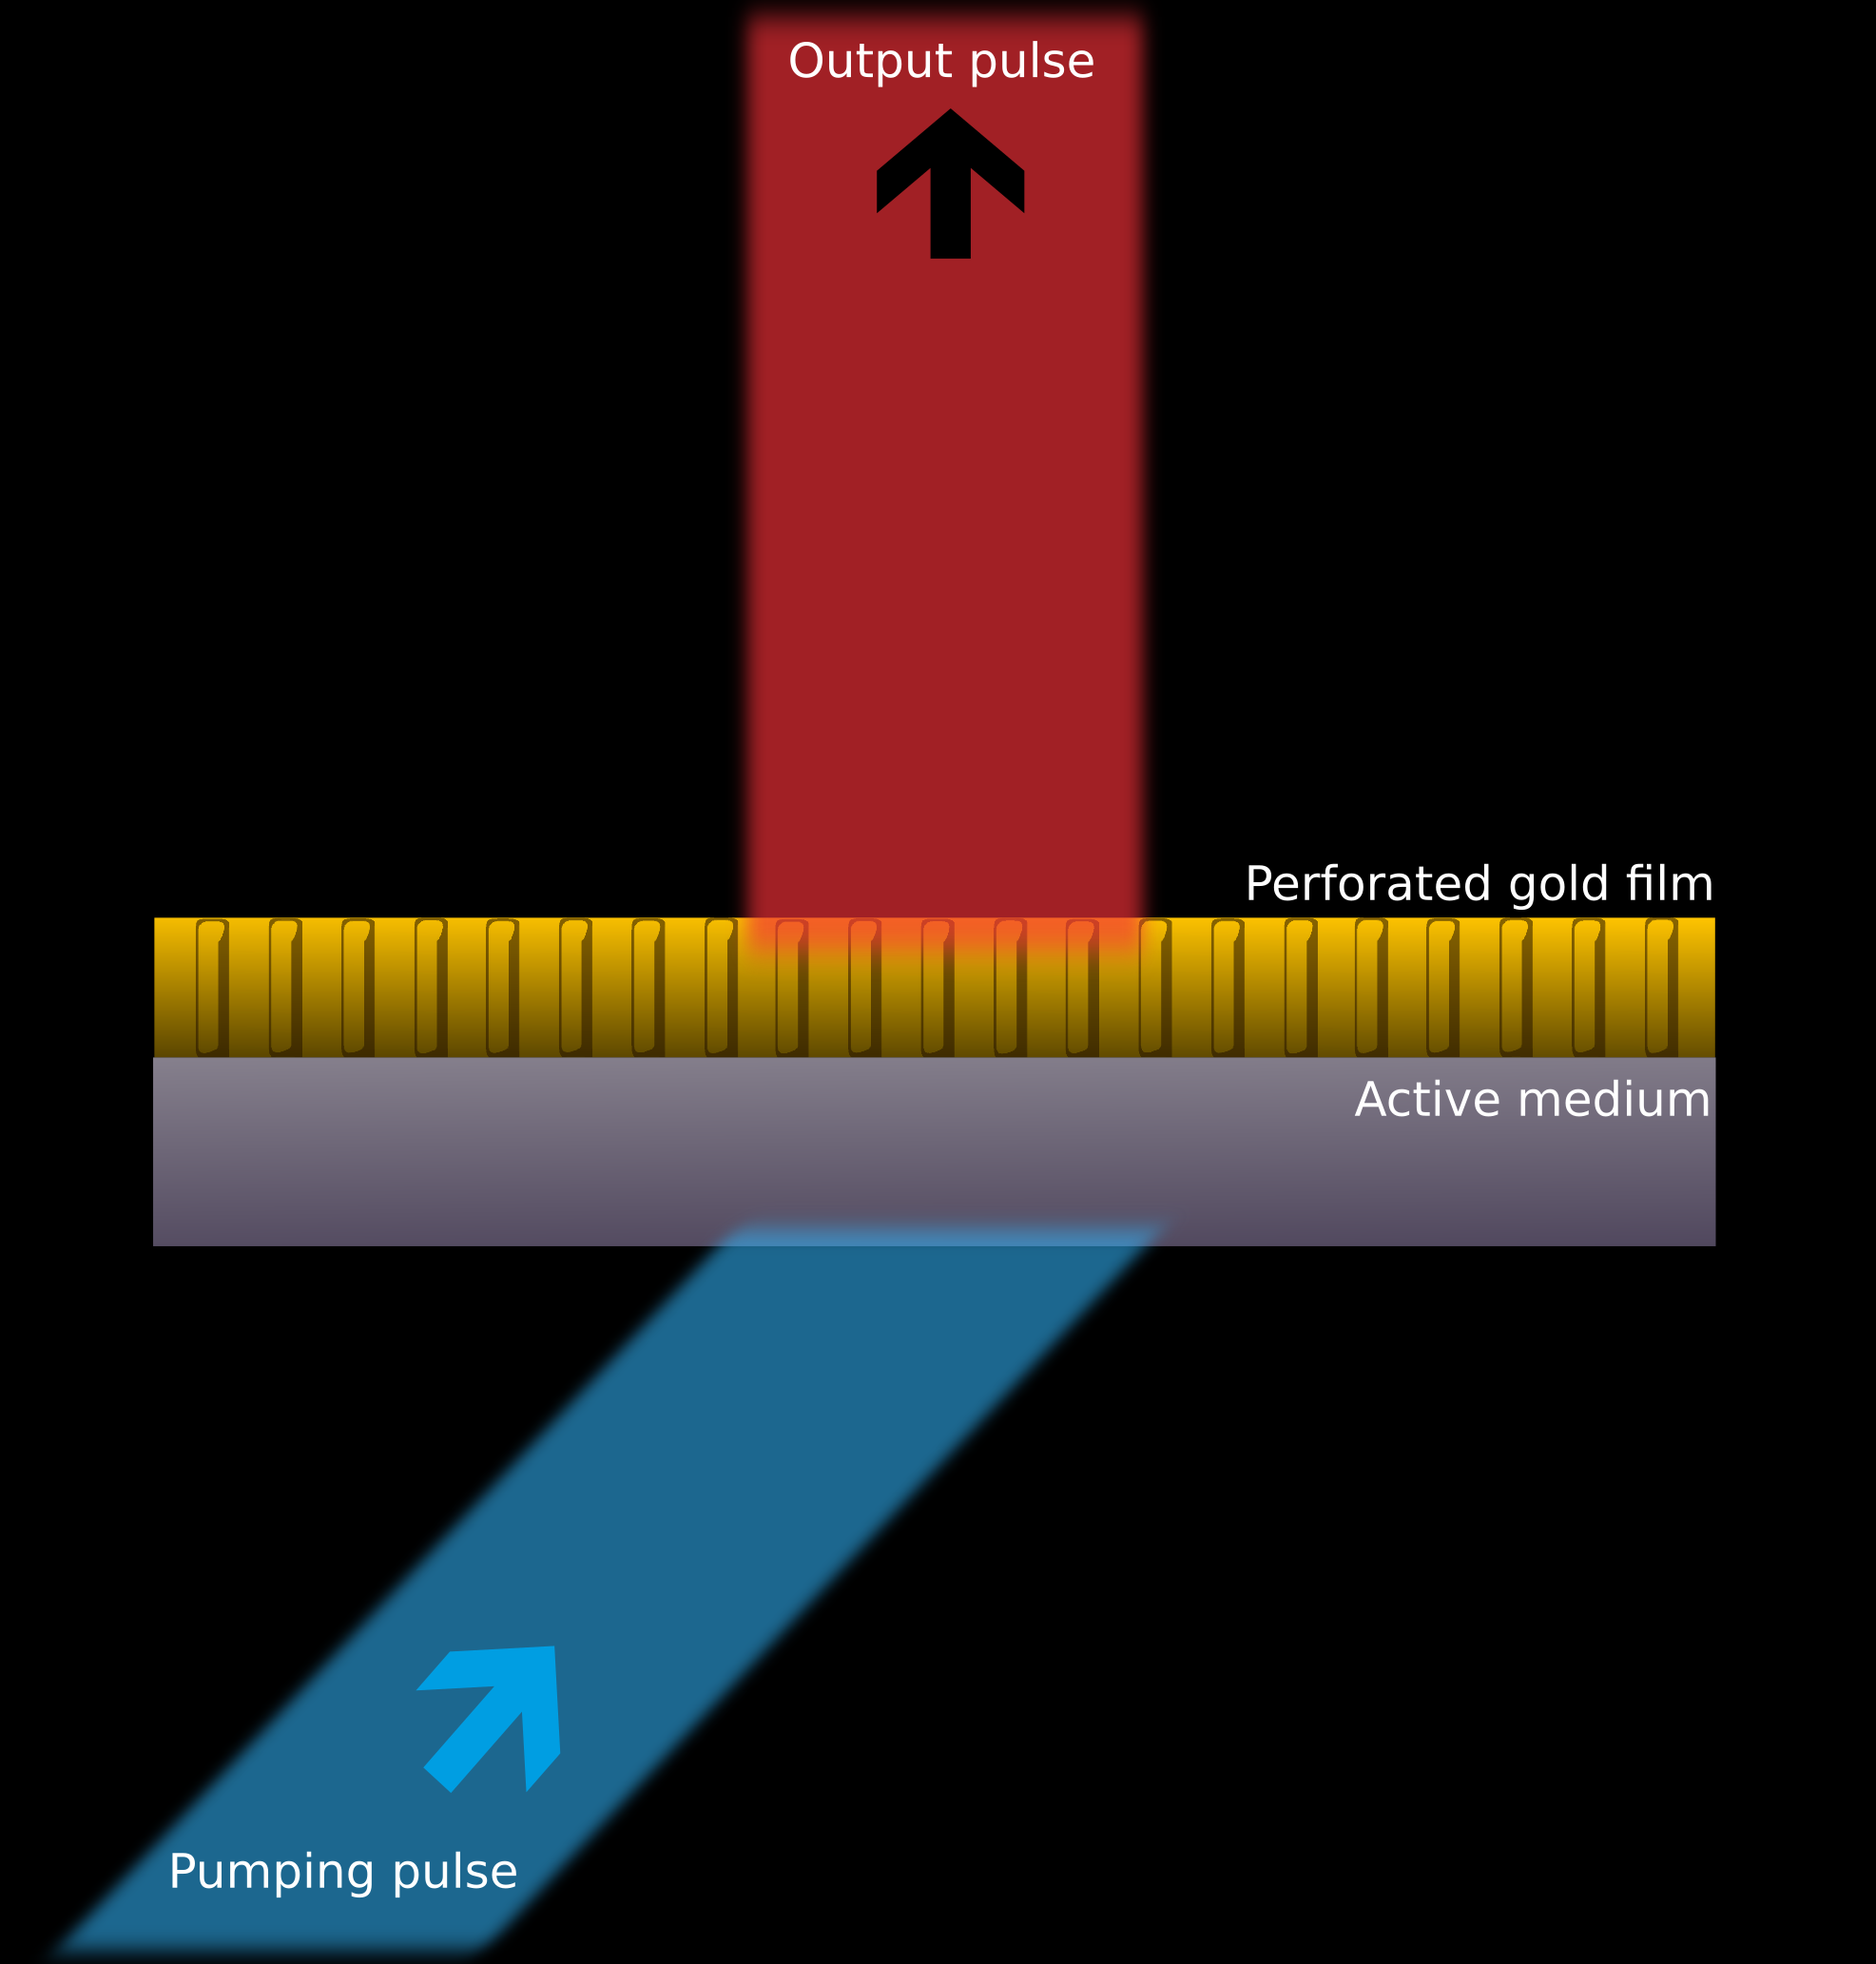
\includegraphics[width=\linewidth]{Fig1.png}
		%\caption{Coffee.}
	\end{subfigure}
	\caption{The sketch of the two-dimensional plasmonic distributed feedback laser. The diameter of the holes is $160$ $\text{nm}$, the distance between holes is $470$ $\text{nm}$, the thickness of the Au film is $100$ $\text{nm}$.}
	\label{fig1}
\end{figure}

\section*{Temporal dynamics of a two-dimensional plasmonic DFB laser}
A conventional plasmonic DFB laser consists of a periodic plasmonic structure, e.g., a metallic film perforated by an array of holes \cite{BeijnumPRL,DorofeenkoOptExp,MengLPR,nefedkin2018acsphot,TennerJOpt,TennerACSPhot,Zyablovsky2017Optimum,Melentiev2017nanolaser} or two-dimensional arrays of plasmonic nanoparticles \cite{ZhouNatNano,SchokkerPRB,daskalakis2018nanolett,SchokkerACSPhot,YangNatComm,YangACSNano,hakala2017lasing,wang2017band}, and an active medium.
The eigenmodes of such a system are Bloch modes which are distributed over the whole surface of the laser.
To overcome losses in the metal, an external pumping (optical or electrical) of the active medium is used.
In the case of optical pumping, the diameter of the pump beam is usually smaller than the size of the periodic plasmonic structure \cite{TennerACSPhot,ZhouNatNano,daskalakis2018nanolett}, see Fig.~\ref{fig1}.
In such a case, the EM field is excited inside the pumped area and is formed by a large number of Bloch modes \cite{TennerACSPhot,nefedkin2018acsphot}.
To describe the multimode dynamics of the plasmonic DFB laser we use an approach which has been proposed in Ref. \cite{Zyablovsky2017approach} for considering ultrafast phenomena in dispersive dissipative media.
This approach is based on the following equations:
\begin{equation}\label{eq1}
\frac{{d{n_{jk}}}}{{dt}} =  - \left( {{\gamma _j} + {\gamma _k}} \right){n_{jk}} + i\left( {{\omega _j} - {\omega _k}} \right){n_{jk}} + \sum\limits_{m=1}^{N_{\text{atom}}} {\left( {{\Omega _{km}}{\varphi _{jm}} + \Omega _{jm}^*\varphi _{km}^*} \right)} 
\end{equation}
\begin{equation}\label{eq2}
\frac{{d{D_m}}}{{dt}} =  - {\gamma _D}\left( {1 + {D_m}} \right)  - 2\sum\limits_{j=1}^{N_{\text{mode}}} {\left( {{\Omega _{jm}}{\varphi _{jm}} + \Omega _{jm}^*\varphi _{jm}^*} \right)} 
\end{equation}
\begin{equation}\label{eq3}
\frac{{d{\varphi _{jm}}}}{{dt}} =  -\gamma_{jm}^{\varphi} {\varphi _{jm}} + i\left( {{\omega _j^a} - {\omega _\sigma }} \right){\varphi _{jm}} + \frac{{\Omega _{jm}^*}}{2}\left( {{D_m} + 1} \right) + \sum\limits_{l=1}^{N_{\text{mode}}} {\Omega _{lm}^*{n_{jl}}{D_m}} , 
\end{equation}
Here, $n_{jj}$ is the photon number in the $j$th Bloch mode, $n_{jk}$ is an interference term responsible for the flow of photons from the $k$th to the $j$th mode, when $j \neq k$.
$D_m$ is the population inversion of the $m$th atom and $\varphi _{jm} = - i \langle \hat{a} _j^{+} \hat{\sigma} _m \rangle$ describes the energy flow between the $m$th atom and $j$th mode.
The parameters $\omega _j$, $\gamma _j$ correspond to the real and imaginary parts of the Bloch modes of plasmonic structure; $\omega _{\sigma}$ and $\gamma _D$ are the atom transition frequency and the relaxation rate of the population inversion of the atoms; $\gamma _{jm}^{\varphi} = \gamma _{\sigma} + \gamma _j + \gamma _D / 2$, $\gamma _{\sigma}$ is the relaxation rate of the phase of the atom polarization.
$\Omega _{jm}$ is the Rabi constant of coupling between the $j$th mode and the $m$th atom which can be expressed as
\begin{equation}\label{eq4SM}
{\Omega _{jm}} =  - {{\bf{d}}_m} \cdot {{\bf{E}}_j}({{\bf{r}}_m})/ \hbar.
\end{equation}
Here ${{\bf{d}}_m}$ is the dipole moment of $m$th atom at the transition frequency and ${{\bf{E}}_j}({{\bf{r}}_m})$  is the electric field `per one quantum' in $j$th Bloch mode at the position $\textbf{r}_m$ of $m$th atom, see Appendix and Section 2 in Suppl.Mat. of \cite{nefedkin2018acsphot}. Every atom of the active medium has its coordinates $\textbf{r}_m$, which determine the Rabi constants of interaction between the atom and the Bloch modes of the plasmonic structure, see Eq.~(\ref{eq4SM}). This allows us to take into account the spatial distribution of the pumping and the population inversion within the active medium. Assuming that the time of the external pump pulse lies in the femtosecond range and is much shorter than all the characteristic times of the plasmonic DFB laser, in our model, the ultrashort pulse pumping is described as the initial condition, $D_m(0)$. For atoms lying inside the pump beam, the value of $D_m(0)$ is proportional to the pumping energy per unit area. The population inversions of the atoms whose coordinates lie outside the pump beam are $-1$ at the initial time. Note that the square of the Rabi constant is inversely proportional of the Bloch mode volume and is proportional of the Purcell factor of the mode (see Appendix).

The Eqs.~(\ref{eq1})--(\ref{eq3}) generalize the rate equations widely used in laser theory \cite{SiegmanLasers}.
In addition to the dynamics of the photon number in each mode and the population inversion of each atom, they describe energy flows between the active medium and the Bloch modes, and the interference between the EM fields of the different modes, $n_{jk}$ \cite{Zyablovsky2017approach}. 

For a quantitative description of the temporal dynamics of a plasmonic DFB laser under pulse pumping, we consider a laser based on an Au film perforated by a periodic array of nanosized holes and coated with the layer of the active medium, see Fig.~\ref{fig1}. We consider that the thickness of the Au film is $100$ $\text{nm}$, the diameter of the holes is $160$ $\text{nm}$, and the distance between holes is $470$ $\text{nm}$. The surface of the entire periodic plasmonic structure is $190 \times 190$ $\mu \text{m}^2$. We consider that the transition frequency of the active medium, $\omega_{\sigma}$, is close to the frequency of the second Bloch condition in the plasmonic structure, i.e. $k_\text{pl}(\omega_{\sigma}) \approx G$, where $k_\text{pl}$ is a wavevector of the mode in the plasmonic structure and $G$ is a reciprocal lattice vector \cite{TennerJOpt,TennerACSPhot,nefedkin2018acsphot}. The linewidth of the active medium is about $100 \text{nm}$. Similar plasmonic DFB lasers have been implemented in a number of experiments \cite{BeijnumPRL,TennerJOpt,TennerACSPhot} and their parameters have been well studied \cite{BeijnumPRL,TennerJOpt,TennerACSPhot,nefedkin2018acsphot}.

The EM field distribution of the Bloch modes of the plasmonic structure have been found within the coupled-mode theory \cite{TennerJOpt,TennerACSPhot,nefedkin2018acsphot} (see also Appendix), which describes the hybridization of modes of the system without holes through scattering on the holes. Scattering amplitudes for these modes have been taken from \cite{TennerJOpt,TennerACSPhot}. The coupled-mode theory with such scattering amplitudes demonstrates a good agreement with the experimental measurement of the band-structure of the plasmonic nanohole array laser \cite{TennerJOpt,TennerACSPhot}.

In numerical simulations, we take into account $468$ Bloch modes which have different distributions of the EM field inside the cell of the plasmonic structure. The step of quantization of the Bloch wavevectors is determined by the size of the periodic plasmonic structure, see \cite{nefedkin2018acsphot} and Suppl.Mat. of \cite{nefedkin2018acsphot}.

Using Eqs.~(\ref{eq1})--(\ref{eq3}), we simulate the time response to an ultrashort pump pulse for different diameters of the pump beam.
In Fig.~\ref{fig2}a the dependence of the photon number on time is shown.
As mentioned in the Introduction, there are three stages of the response of the system.
In the first stage, the response of the system is determined by the spontaneous emission in the active medium.
The photon number in the plasmonic DFB laser is small.
For the system under consideration, the duration of this stage, i.e. the delay time, turns out to be less than a picosecond.
In the second stage, the photon number in the plasmonic laser rapidly increases due to stimulated emission in the active medium.
This growth ceases with the saturation of the population inversion in the active medium.
In the third stage, the photon number in the system decreases exponentially with time.
We identify the total response time with the time when the number of photons in the system has decreased by a factor of ten from its maximum value.
This time is about one picosecond.
  
\begin{figure}[h]
	\centering
	\begin{subfigure}[h]{0.45\linewidth}
		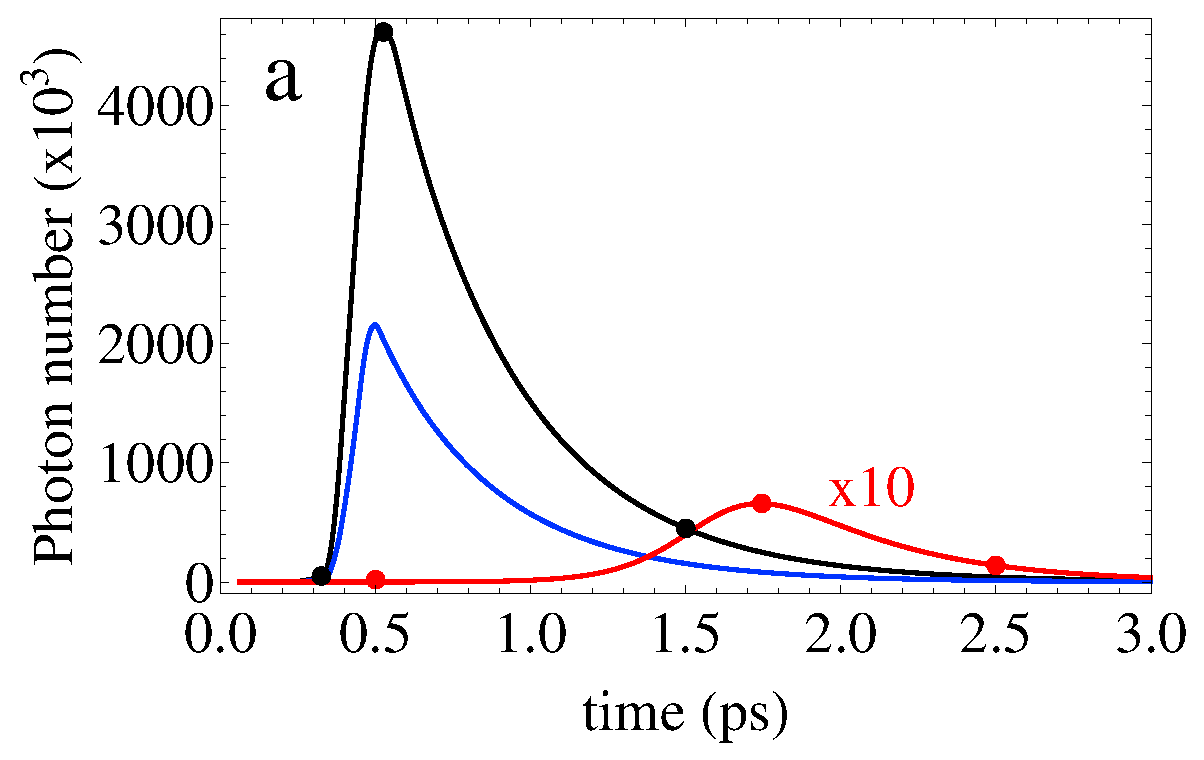
\includegraphics[width=\linewidth]{Fig2a.eps}
		%\caption{}
	\end{subfigure}
	\begin{subfigure}[h]{0.45\linewidth}
		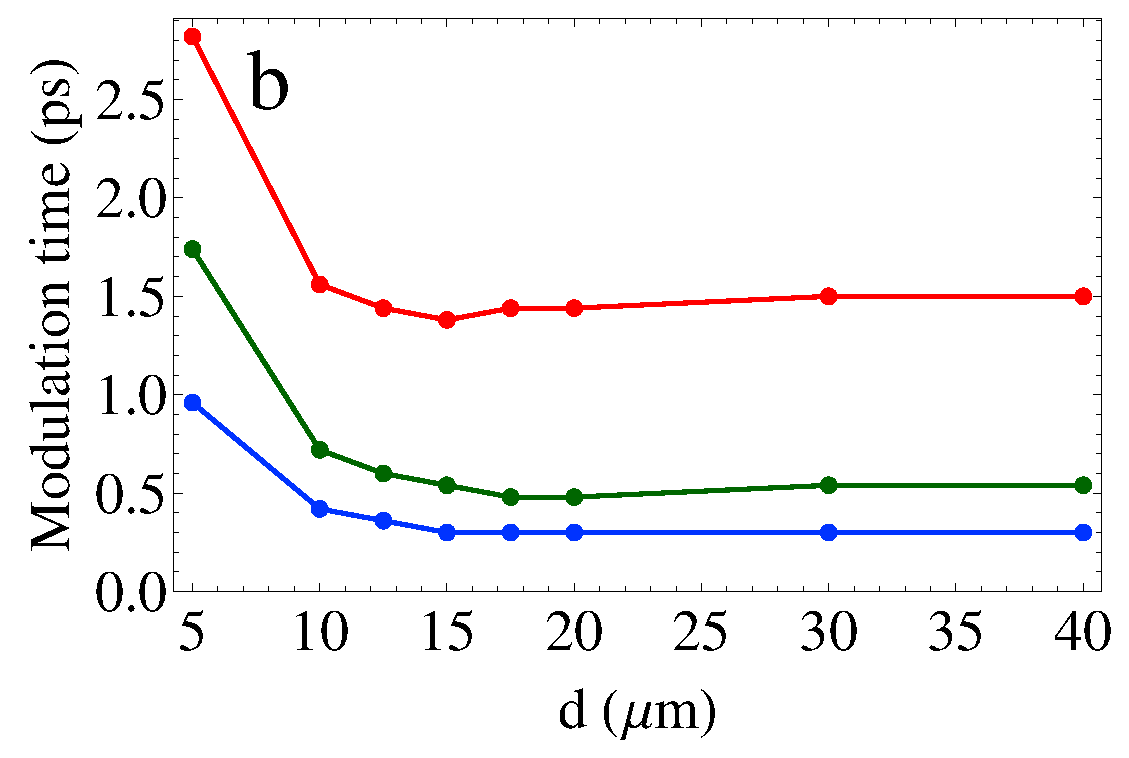
\includegraphics[width=\linewidth]{Fig2b.eps}
		%\caption{}
	\end{subfigure}
	\caption{(a) The dependence of the total photon number on the time at the different diameters of the pump beam. The diameters are equal to 20 $\mu$m (black line), 10 $\mu$m (blue line), and 5 $\mu$m (red line). (b) The dependence of the modulation times on the diameters of the pump beam. The blue line depicts the delay time; the green line depicts the time of the end of the second stage; the red line depicts the total response time.}
	\label{fig2}
\end{figure}

\begin{figure}[h]
	\centering
	\begin{subfigure}[h]{0.32\linewidth}
		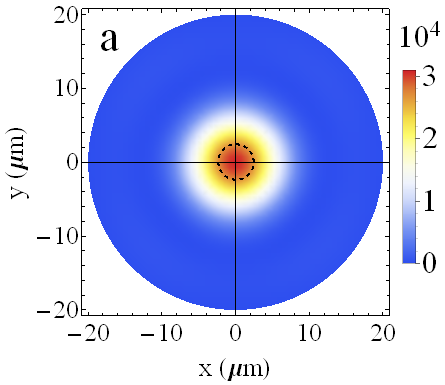
\includegraphics[width=\linewidth]{Fig3a.png}
%		\caption{}
	\end{subfigure}
	\begin{subfigure}[h]{0.32\linewidth}
		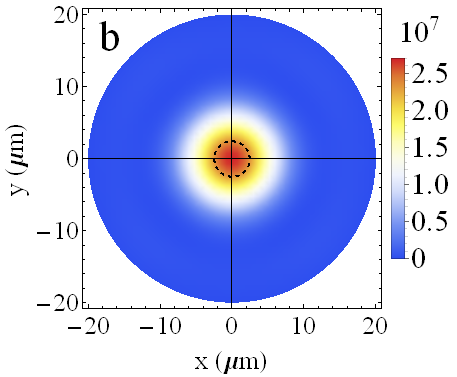
\includegraphics[width=\linewidth]{Fig3b.png}
%		\caption{}
	\end{subfigure}
	\begin{subfigure}[h]{0.32\linewidth}
		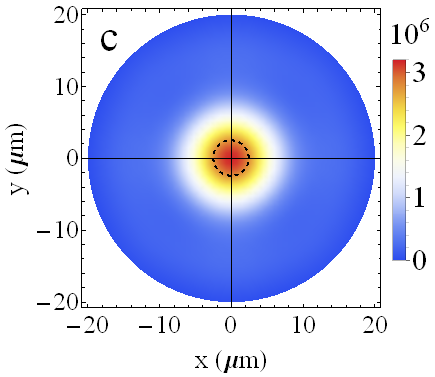
\includegraphics[width=\linewidth]{Fig3c.png}
%		\caption{}
	\end{subfigure}
	\\
	\begin{subfigure}[h]{0.32\linewidth}
		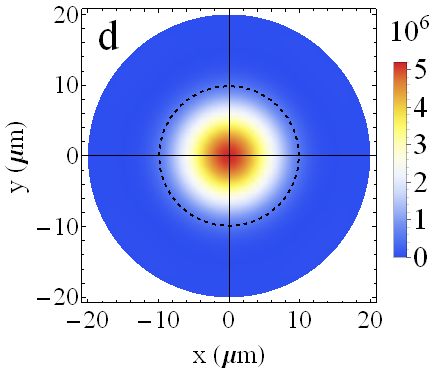
\includegraphics[width=\linewidth]{Fig3d.png}
%		\caption{}
	\end{subfigure}
	\begin{subfigure}[h]{0.32\linewidth}
		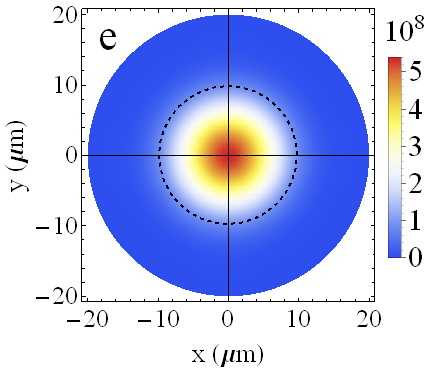
\includegraphics[width=\linewidth]{Fig3e.png}
%		\caption{}
	\end{subfigure}
	\begin{subfigure}[h]{0.32\linewidth}
		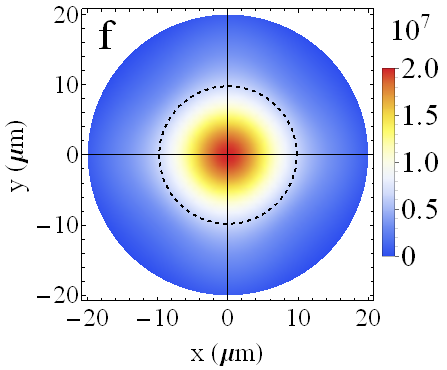
\includegraphics[width=\linewidth]{Fig3f.png}
%		\caption{}
	\end{subfigure}
	\caption{Distribution of the EM field intensity on the surface of the plasmonic DFB laser when the diameter of the pump beam $d_{\text{beam}}<d_{\text{beam}}^*$ (a)-(c) in time moment 0.5 ps (a); 1.75 ps (b); 2.5 ps (c). Distribution of the EM field intensity on the surface of the plasmonic DFB laser when the diameter of the pump beam $d_{\text{beam}}>d_{\text{beam}}^*$ (d)-(f) in time moment 0.32 ps (d); 0.541 ps (e); 1.5 ps (f). These time moments correspond to circles on the red curve and the black curve in Fig.\ref{fig2}a, respectively. The dashed circles denote the boundaries of the pump beam.}
	\label{fig3}	
\end{figure}

The dependence of the total photon number on time is qualitatively the same for different diameters of the pump beam.
However, the response times manifest a non-monotonic dependence on the size of the pump beam, see Fig.~\ref{fig2}b.
It can be seen that there is a critical size of the pump beam at which the response time is a minimum.
For the considered plasmonic DFB laser, the critical diameter of the pump beam is about 15 $\mu$m.
As the pump beam diameter decreases, the response time increases rapidly.
With an increase in the diameter of the pump beam, the response time changes slowly.
This kind of behavior of the plasmonic DFB laser takes place at different initial values of the population inversion of the active atoms.
Thus, there is a diameter of the pump beam, $d_{\text{beam}}^*$, at which an ultrafast light modulation in the plasmonic DFB laser is achieved.

\section*{Single-mode approximation}

The existence of a critical size of the pump beam can be explained with the example of a single-mode model. To justify the single-mode approximation, we calculate the distribution of the electric field intensity over the area of the plasmonic DFB laser at different moments of time, see Fig.~\ref{fig3}.
In our simulations we take into account several hundred of the Bloch modes of the plasmonic structure, which together form the EM field distribution in the active medium. One can see that this distribution does not change in the first and second stages of the system response. In other words, there is a dynamical balance between relaxation processes in the plasmonic structure, the propagation of the EM field outside the pumped area and the stimulated amplification of the EM field inside the pumped area. When the diameter of the pump beam is larger than the critical value, $d_{\text{beam}} > d_{\text{beam}}^*$, the electric field is located inside the pumped region of the active medium, see Figs.~\ref{fig3}(d)--(f).
In the opposite case, when $d_{\text{beam}} < d_{\text{beam}}^*$, the main part of the electric field is outside the pumped area, see Figs.~\ref{fig3}(a)--(c).
However, in both cases, the spatial distribution of the electric field intensity remains almost unchanged during its temporal evolution. 

We use the fact of the constancy of the EM field distribution to construct a single-mode model. To do this, we assume that there is a single collective mode, the EM field distribution of which coincides with the EM field distribution found in the numerical simulations of the multimode problem. Furthermore, we assume that the pumped active medium interacts only with such a single collective mode. Within these approximations, the system dynamics can be described by the following system of equations \cite{SiegmanLasers}:
\begin{gather} 
\dot n =  - 2{\gamma _a}n + 2{N_{\text{at}}}{\Omega _R}\varphi \label{ZE1}
\\
\dot \varphi = - \left( {{\gamma _a} + {\gamma _\sigma }} \right)\varphi + {\Omega _R}\left( {2nD + D + 1} \right)/2 \label{ZE2}
\\
\dot D =  - {\gamma _D}\left( {D + 1} \right) - 4{\Omega _R}\varphi, \label{ZE3}
\end{gather}
where $n$ is the number of photons in the collective mode, $D$ is the mean population inversion of pumped atoms of the active medium, $\varphi$ describes the mean energy flow from the active medium to the collective mode, and $N_{\text{at}}$ is the number of atoms of the active medium lying in the collective mode.
We suppose that the relaxation rate of the EM field in the collective mode is equal to the characteristic relaxation rate of the modes of the plasmonic structure, i.e., $\gamma_a \simeq 10^{12} \text{s}^{-1}$.
Note that the finite size of the pump beam can lead to the appearance of edge effects and influence on the mode quality factor, see \cite{hakala2017lasing}.
In the single-mode model, we do not take into account these effects.
The typical relaxation rate of the population inversion of the active medium is $\gamma_D \simeq 10^9 \text{s}^{-1}$ while the phase relaxation rate is $\gamma_{\sigma}\simeq 10^{13} \text{s}^{-1}$.
Thus, the phase relaxation rate is much larger than other relaxation rates, $\gamma_\sigma \gg \gamma_a, \gamma_D$.
For this reason, one can adiabatically eliminate $\varphi$ from Eqs.~(\ref{ZE1})--(\ref{ZE3}) and obtain the conventional rate equations
\begin{gather} 
\dot n =  - 2 {\gamma _a}n + {N_{\text{at}}}\Omega _R^2\left( {2nD + D + 1} \right)/{\gamma _\sigma } \label{RE1}
\\
\dot D =  - {\gamma _D}\left( {D + 1} \right) - 2\Omega _R^2\left( {2nD + D + 1} \right)/{\gamma _\sigma } \label{RE2}
\end{gather}
As initial condition we take $D(0) = 1$ and $n(0) = 0$, i.e., all atoms are inverted and there are no photons in the mode.
The temporal dynamics of such a system is well-known \cite{SiegmanLasers}; it is shown in Fig.~\ref{fig4}.

\begin{figure}[h]
	\centering
	\begin{subfigure}[h]{0.45\linewidth}
		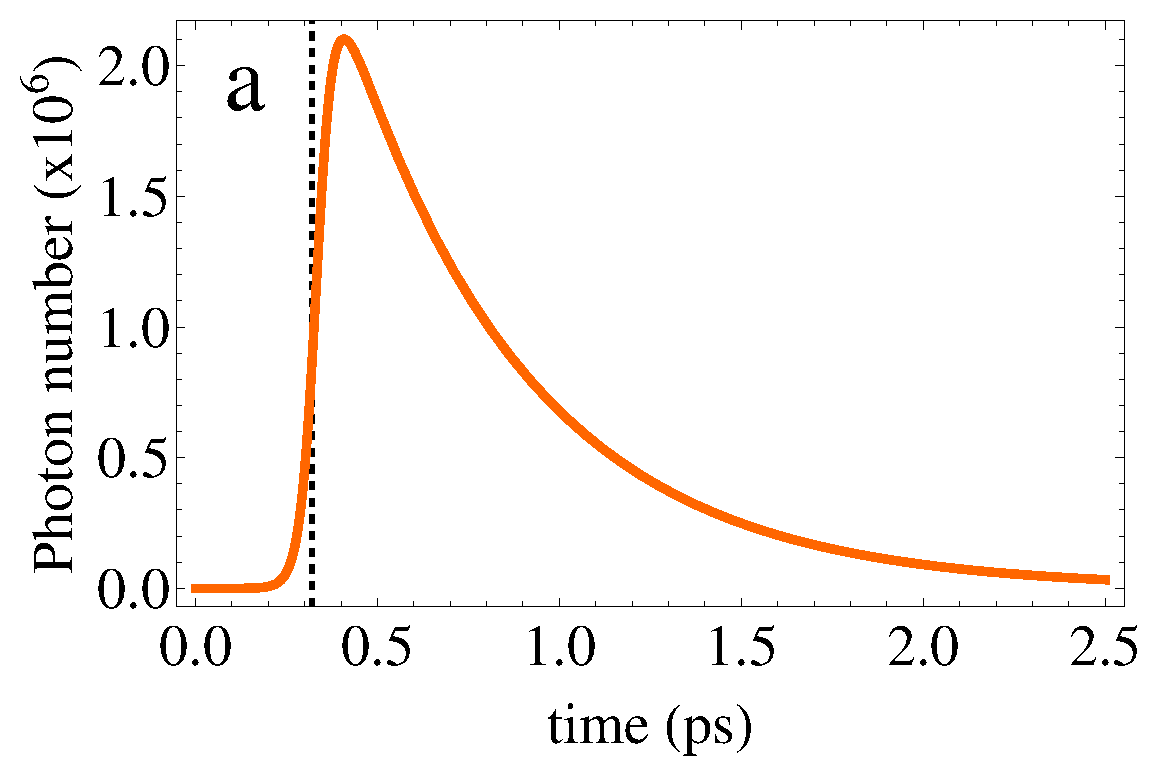
\includegraphics[width=\linewidth]{Fig4a.eps}
		%\caption{}
	\end{subfigure}
	\begin{subfigure}[h!]{0.45\linewidth}
		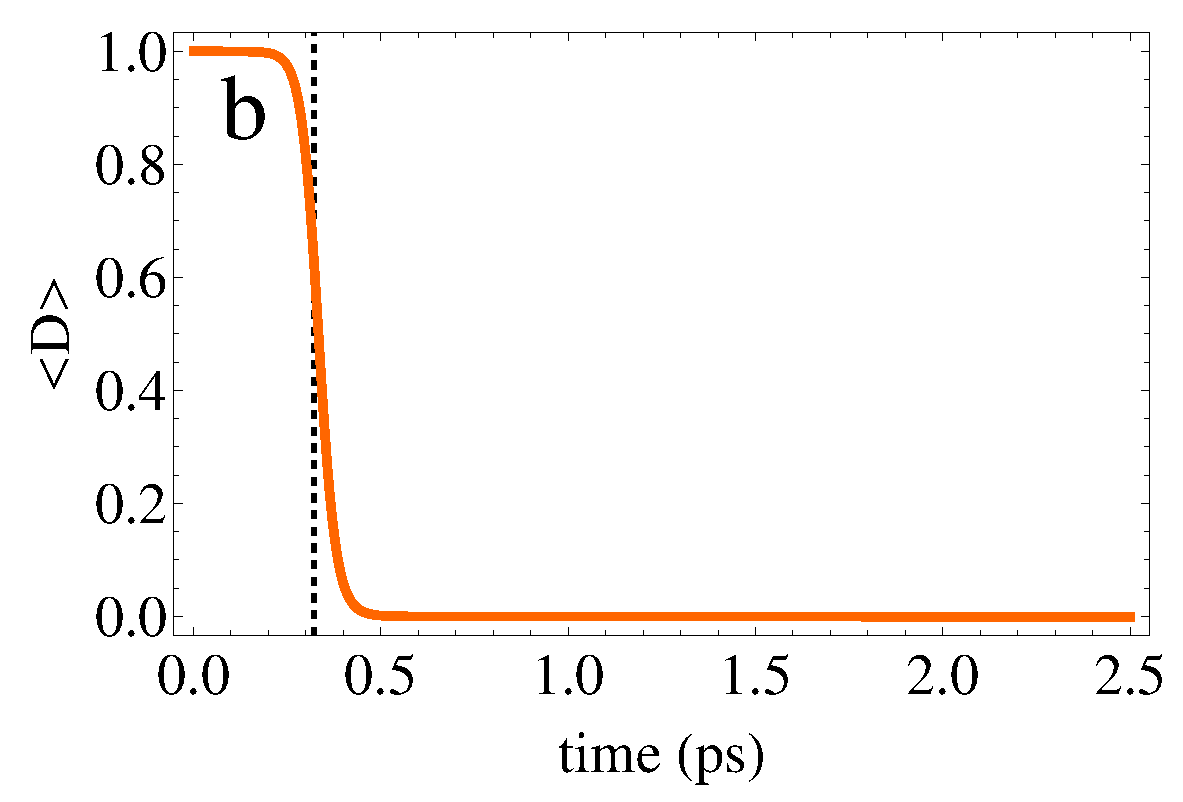
\includegraphics[width=\linewidth]{Fig4b.eps}
		%\caption{}
	\end{subfigure}
	\caption{The dependences of the photon number (a) and the population inversion of atom (b) on time obtained from the single-mode model, Eqs. (\ref{RE1})-(\ref{RE2}); the vertical dashed lines denote the delay time, $t_{\text{delay}}$, obtained with Eq. (\ref{tdel}).
	}
	\label{fig4}
\end{figure}

The dynamics of the photon number in the collective mode obtained with Eqs.~(\ref{RE1})--(\ref{RE2}) is similar to the behavior of the total photon number in the real plasmonic DFB laser, cf.  Fig.~\ref{fig4}a and Fig.~\ref{fig2}a.
We observe three stages of the laser response, which are quantitatively similar to the stages in the real plasmonic DFB laser.

In the first stage, $D$ is constant and $n$ reaches stationary states at fixed $D$.
Under this assumption the solution of Eq.~(\ref{RE1}) is
\begin{equation} 
n\left( t \right) = \frac{{{N_{\text{at}}}\Omega _R^2\left( {D + 1} \right)/{\gamma _\sigma }}}{{2{N_{\text{at}}}\Omega _R^2D/{\gamma _\sigma } - 2 {\gamma _a}}}\left( {\exp \left[ 2\left( {{N_{\text{at}}}\Omega _R^2D/{\gamma _\sigma } - {\gamma _a}} \right)t \right] - 1} \right) = \frac{{\xi \left( {D + 1} \right)}}{{2\left( {\xi-1} \right)}}\left( {\exp \left[\left( {\xi D - 1} \right) 2 {\gamma _a}t \right] - 1} \right), \label{ph}
\end{equation}
where $\xi={{N_{\text{at}}}\Omega _R^2D/{\gamma _\sigma \gamma_a }}$ is the inverse threshold value of the pumping in the continuous-wave (CW) regime \cite{ScullyQO}.
At the initial moment, $D \simeq 1$ and we have  
\begin{equation} 
n\left( t \right) = \frac{\xi }{{\left( {\xi - 1} \right)}}\left( {\exp \left[ \left( {\xi  - 1} \right) 2 {\gamma _a}t \right] - 1} \right). \label{ph0}
\end{equation}
Substituting Eq.~(\ref{ph0}) into Eq.~(\ref{RE2}) one obtains
\begin{equation} 
\dot D =  - {\gamma _D}\left( {1 + \eta } \right)\left( {D + 1} \right) - {\gamma _D}\frac{{2\xi \eta D}}{{\left( {\xi  - 1} \right)}}\left( {\exp \left[\left( {\xi  - 1} \right) 2 {\gamma _a}t \right] - 1} \right), \label{inv0}
\end{equation}
where we have put $\eta = 2 \Omega_R^2 /\gamma_D \gamma_\sigma$. 

The second stage corresponds to the time when the exponential term in Eq.~(\ref{inv0}) is dominant, and the dynamics is strongly nonlinear.
This nonlinear term describes the stimulated energy flow from the atoms to the collective mode.
In this case, from Eq.~(\ref{inv0}) we obtain the equation
\begin{equation} 
\dot D =  - {\gamma _D}\frac{{2\xi \eta D}}{{\left( {\xi  - 1} \right)}} \exp \left[\left( {\xi  - 1} \right) 2 {\gamma _a}t \right] \label{invnl1}
\end{equation}
which has the solution
\begin{equation} 
D(t) \simeq \exp \left(  - \frac{{\xi \eta {\gamma _D}}}{{{\left( {\xi  - 1} \right)}^2}{\gamma _a}}  \exp \left[\left( {\xi  - 1} \right) 2 {\gamma _a}t \right] \right) = \exp \left(  - \frac{{{\xi ^2}}}{{{N_{\text{at}}}{{\left( {\xi  - 1} \right)}^2}}}\exp \left[\left( {\xi  - 1} \right) 2 {\gamma _a}t \right] \right).
\end{equation}
The characteristic time for $D$ to change is 
\begin{equation} 
{t_{delay}} = (2\gamma _a)^{ - 1}{\left( {\xi  - 1} \right)^{ - 1}}\ln \left( {{N_{\text{at}}}{{\left( {\xi - 1} \right)}^2}/{\xi ^2}} \right). \label{tdele}
\end{equation}
At this time, a sharp decrease of $D$ appears, see Fig.~\ref{fig4}b.
Note that the assumption that the evolution of $D$ is much slower than the evolution of $n$ is valid when $t_{delay} \gg \gamma_a^{-1} \xi^{-1}$, i.e., $\ln \left( {{N_{\text{at}}}{{\left( {\xi  - 1} \right)}^2}/{\xi ^2}} \right) \gg 1$.
When $\xi \gg 1$, the assumption is correct if $N_{\text{at}} \gg 1$, which is true for the considered system.

For $\xi \gg 1$, Eq.~(\ref{tdele}) simplifies to  
\begin{equation} 
{t_{\text{delay}}} = {\gamma _\sigma }\ln \left( {{N_{\text{at}}}} \right)/2{N_{\text{at}}}\Omega _R^2. \label{tdel}
\end{equation}

\begin{figure}[h]
	\centering
	\begin{subfigure}[h]{0.45\linewidth}
		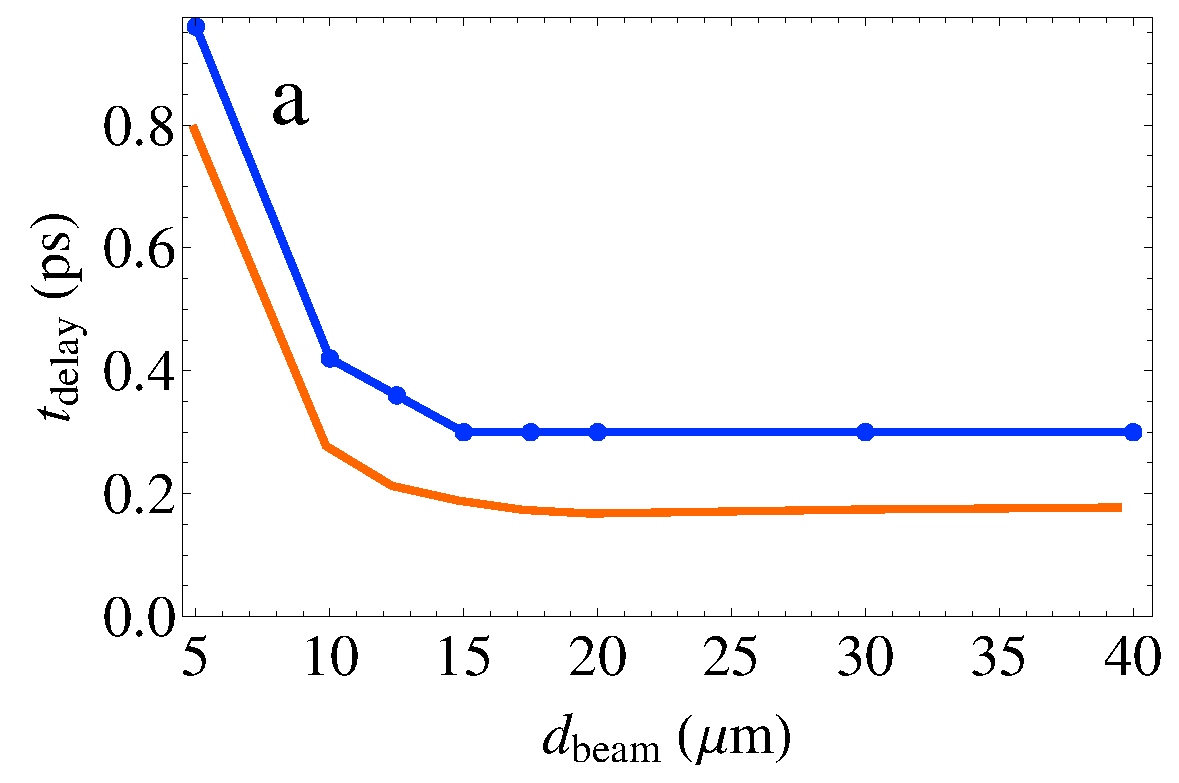
\includegraphics[width=\linewidth]{Fig5a.eps}
		%\caption{}
	\end{subfigure}
	\begin{subfigure}[h]{0.45\linewidth}
		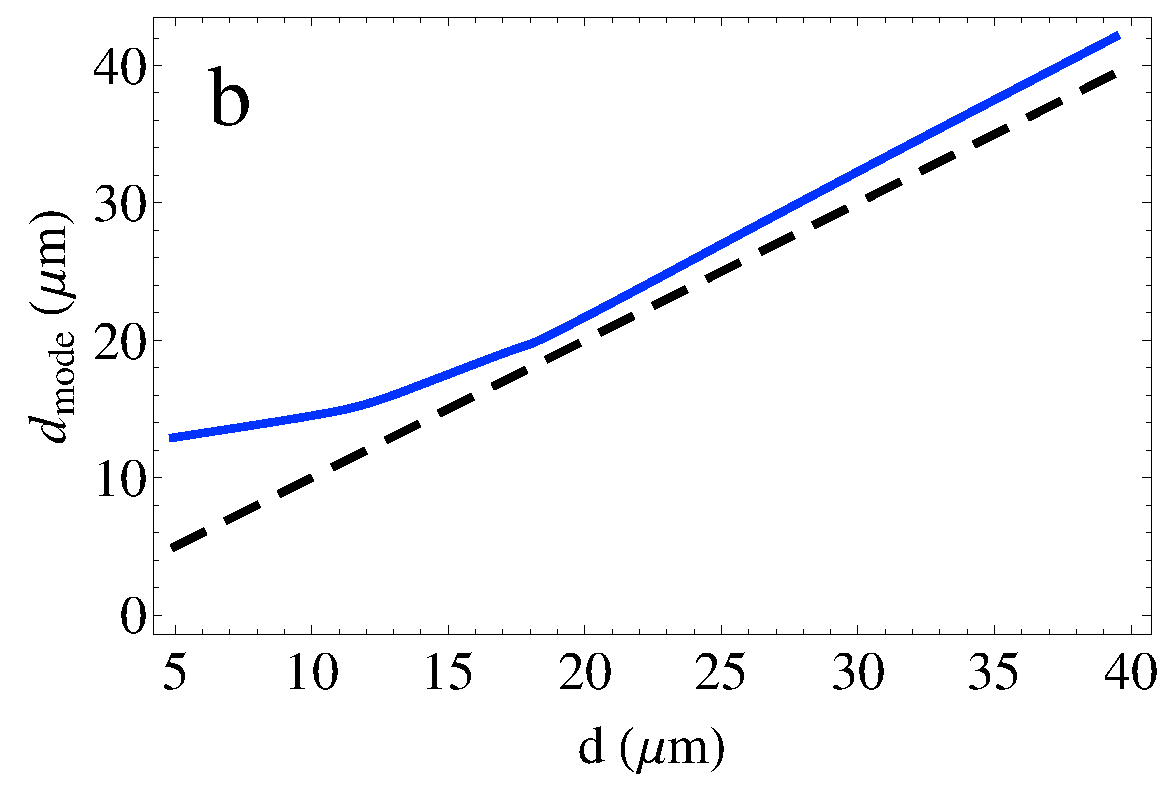
\includegraphics[width=\linewidth]{Fig5b.eps}
		%\caption{}
	\end{subfigure}
	\caption{(a) The dependence of the delay time on the pump beam diameter. The blue solid line is obtained from numerical simulation of Eqs. (\ref{eq1})--(\ref{eq3}), the orange thick line is obtained from Eq. (\ref{tdel}). (b) The dependence of the diameter of the collective mode on the pump beam diameter (blue line). The black dashed line denotes the pump beam diameter.
	}
	\label{fig5}
\end{figure}

The figure \ref{fig5}a shows that the analytical approximation, Eq.~(\ref{tdel}), agrees well with the numerical simulation of the exact model, Eqs. (\ref{eq1})--(\ref{eq3}).
Let us analyze the dependence of the delay time, Eq.~(\ref{tdel}), on the size of the pumped area.
The number of atoms depends quadratically on the diameter $d_{\text{beam}}$ of the pump beam, i.e., $N_{\text{at}} \sim d_{\text{beam}}^2$.
In turn, the square of the Rabi constant is inversely proportional to the square of the diameter $d_{\text{mode}}^2$ of the collective mode, i.e., $\Omega_{R}^{2} \sim 1/d_{\text{mode}}^2$.
So, we have $t_{\text{delay}} \sim d_{\text{mode}}^2\ln \left( d_{\text{beam}}^2 \right ) /d_{\text{beam}}^2$.
The dependence of $d_{\text{mode}}$ on $d_{\text{beam}}$ is shown in Fig.~\ref{fig5}b.

It can be seen that there is a critical value, $d_{\text{beam}}^*$, of the diameter of the pump beam, which divides two different cases.
When $d_{\text{beam}}>d_{\text{beam}}^*$, the electric field of the collective mode is localized inside the pump beam, see Figs.~\ref{fig3}(d)--(f).
As a consequence, the mode diameter is proportional to the beam diameter, i.e., $d_{\text{mode}} \sim d_{\text{beam}}$, see Fig.~\ref{fig5}b.
For this case, from Eq.~(\ref{tdel}) we have $t_{\text{delay}} \sim \ln d_{\text{beam}}$.
This dependence is in agreement with a slow growth of the delay time of the DFB laser, see Fig\ref{fig2}b.
When $d_{\text{beam}}<d_{\text{beam}}^*$, the electric field of the collective mode is localized outside the pump beam, see Figs.~\ref{fig3}(a)--(c), and the mode size is determined by the characteristic propagation length of the EM field in the unpumped region.
As a result, the mode diameter does not depend on the beam diameter, and $d_{\text{mode}} \sim \text{const}$, see Fig.~\ref{fig5}b.
In this case, $t_{\text{delay}} \sim \ln(d_{\text{beam}}^2)/d_{\text{beam}}^2$.
This is in agreement with an increase of the delay time  when the pump beam diameter of the plasmonic DFB laser is reduced, see Fig.~\ref{fig2}b.
Note that the critical value $d_{\text{beam}}^*$ corresponds to the characteristic propagation length of the EM field outside the pumped active medium and may be evaluated as $d_{\text{beam}}^* \sim v_{\text{group}}/\gamma_a$.
For the parameters of the DFB laser we have $d_{\text{beam}}^* \sim 10 \mu \text{m}$, which is in agreement with the full model, Fig.~\ref{fig2}b.
Thus, because the delay time grows when $d_{\text{beam}}>d_{\text{beam}}^*$ and grows in the opposite case as well, we come to the conclusion that there is a critical value, $\sim d_{\text{beam}}^*$, for the diameter of the pump beam for which the response time is a minimum.

\section*{Conclusion}

To summarize, we have studied the temporal dynamics of a two-dimensional plasmonic DFB laser under ultrashort pulse pumping.
Relying on numerical simulations and analytical calculations, we have shown that the response time of such a laser for experimental parameters from ~\cite{TennerJOpt,TennerACSPhot} can be decreased to one picosecond, which corresponds to a modulation frequency of $1$ THz.
This value is close to the upper limit for plasmonic lasers (the total response time can not be shorter than the time of the third stage, which is determined by the losses in the cavity, and is $ \sim 1$ ps).

It has been shown that the laser's response time can be shortened by optimizing the size of the pump beam, as a result of the consequent reduction of the delay time.
The dependence of the response time on the size of the pump beam is for following reason.
The interaction of the laser modes with the pumped active medium results in the emergence of a single collective mode.
If the size of the pump beam exceeds the propagation length of the EM waves, this collective mode is located in the pumped area.
The response time then grows logarithmically with increasing pump beam diameter.
In contrast, when the mode is outside the pumped region, the response time is approximately inversely proportional to the square of the pump beam diameter, and so increases rapidly as this diameter decreases from its critical value.
It is interesting to note that the delay time, Eq.~(\ref{tdel}), resembles the dependence of the delay time of a superradiant burst \cite{gross1982superradiance, andreev1980collective,nefedkin2017badcavitySR}.
Indeed, it is well known \cite{gross1982superradiance, andreev1980collective} that a system consisting of initially inverted atoms placed in a low-Q cavity, i.e., when $\gamma_a \gg \gamma_D$, exhibits a superradiant burst with the delay time, Eq.~(\ref{tdel}). In the plasmonic cavity, the inequality $\gamma_a \gg \gamma_D$ is always hold true and, for this reason, the superradiance problem and the problem that we investigate here have the same physical grounds. Further study of the relationship between these problems may be important in the context of creating ultrafast optoelectronic devices.

In consequense, there is the diameter of the pump beam, $d_{\text{beam}}^*$, necessary to achieve the short response time. This diameter is about the decay length of the EM field in the plasmonic structure and for the considered plasmonic laser is $\sim 15 \mu$m. The existence of the critical pump beam size gives the opportunity to reduce the energy consumption because further increase of the pump beam size does not shorten the response time.
In turn, if the area of the pump beam is small, there is the opportunity to reduce the size of the device.
Thus, the obtained results pave the way to creating ultrafast optoelectronic devices based on plasmonic lasers with low power consumption which have the potential of on-chip integration.

\section*{Acknowledgements}

The reported study was funded by RFBR according to the research project No. 18-32-00596.

\section*{Appendix}
To find the electric field ${{\bf{E}}_j}({{\bf{r}}_m})$  'per one quantum', we equate the energy of one quantum to the energy of the EM field in the resonator:
\begin{equation}
\hbar {\omega _j} = \frac{1}{{8\pi }}\int\limits_V {\left( {{{\left. {\frac{{\partial {\mathop{\rm Re}\nolimits} \left( {\varepsilon(\omega, \textbf{r}) \omega } \right)}}{{\partial \omega }}} \right|}_{\omega  = {\omega _j}}}{{\left| {{{\bf{E}}_j}\left( {\bf{r}} \right)} \right|}^2} + {{\left| {{{\bf{H}}_j}\left( {\bf{r}} \right)} \right|}^2}} \right){d^3}{\bf{r}}} \tag{A.1}
\end{equation}
where $\varepsilon (\omega, \textbf{r})$  is the dielectric constant.

In a two-dimensional periodic plasmonic structure whose surface is parallel to the $xy$-plane, the electric and magnetic fields satisfy the Bloch condition,
\begin{equation}
{{\bf{E}}_j}\left( {\bf{r}} \right) = {A_{0j}}\exp \left( {i{k_{xj}}x + i{k_{yj}}y} \right){{\bf{e}}_j}\left( {x,y,z} \right) \tag{A.2}
\end{equation}
\begin{equation}
{{\bf{H}}_j}\left( {\bf{r}} \right) = {A_{0j}}\exp \left( {i{k_{xj}}x + i{k_{yj}}y} \right){{\bf{h}}_j}\left( {x,y,z} \right), \tag{A.3}
\end{equation}
where $A_{0j}$ is a real normalization constant for \textit{j}th mode; ${{\bf{e}}_j}\left( {x,y,z} \right) = {{\bf{e}}_j}\left( {x + {L_x},y + {L_y},z} \right)$  and ${{\bf{h}}_j}\left( {x,y,z} \right) = {{\bf{h}}_j}\left( {x + {L_x},y + {L_y},z} \right)$, $L_x$ and $L_y$ are periods of the plasmonic structure along $x$-axis and $y$-axis, respectively.

The functions ${{\bf{e}}_j}\left(\textbf{r}\right)$ and ${{\bf{h}}_j}\left(\textbf{r}\right)$ can be found within the couple-mode theory, see \cite{TennerJOpt,TennerACSPhot} and Section 2 in Suppl.Mat of \cite{nefedkin2018acsphot}. In this approach, the eigenmodes of the plasmonic structure with holes are expressed as linear combinations of the eigenmodes of the plasmonic structure without holes \cite{TennerJOpt,TennerACSPhot}. The expansion coefficients are calculated through the scattering matrix which contains the scattering amplitudes at angles $0^{\circ }$, $\pm 90^{\circ }$ and $180^{\circ }$ and effective refractive index of the plasmonic structure \cite{TennerJOpt,TennerACSPhot}.

The eigenmodes of the plasmonic structure without holes are TM-modes, similar to surface plasmons at the metal-dielectric interface \cite{TennerJOpt,TennerACSPhot}. 
These modes have an in-plane component of the magnetic field, $h_{\parallel}$, which is perpendicular to the direction of mode's propagation and both out-of-plane, $e_{\perp}$, and in-plane, $e_{\parallel}$, components of the electric field \cite{TennerJOpt,TennerACSPhot}. 
The in-plane electric field, $e_{\parallel}$, is in the direction of the mode's propagation. 
The out-of-plane component of the electric field, $e_{\perp}$, is much greater than the in-plane component, $e_{\parallel}$ \cite{TennerJOpt,TennerACSPhot} and so it plays the main role in the interaction of the modes with the active medium.

The eigenmodes of the plasmonic structure with the holes have been found within the coupled-mode theory with the experimental values of the scattering amplitudes, see~\cite{TennerJOpt,TennerACSPhot} and Section 2 in Suppl.Mat. of \cite{nefedkin2018acsphot}. The coupled-mode theory with such scattering amplitudes demonstrates a good agreement with the experimental measurement of the band-structure of the plasmonic nanohole arrays laser \cite{TennerJOpt}.
Near the transition frequency of the active medium, there are four different dispersion curves. The eigenmodes corresponding to different dispersion curves have various radiation losses and EM field distributions inside the unit cell of the plasmonic structure (see \cite{TennerJOpt,TennerACSPhot} and Section 2 in Suppl.Mat. of \cite{nefedkin2018acsphot}). In particular, at the edge of the band gap, when the Bloch wavevectors $\left(k_{xj}, k_{yj}\right) = \left(0, 0\right)$, the EM field distributions in the modes from the different dispersion curves are 

\textbf{Table A}

$\begin{array}{cccc}
\text{The number of the dispersion curve} & e_{\parallel} & \
h_{\parallel} & \
e_ {\perp } \left( e_z \right) \\
\text{1} & \sin (G x)+\sin (G y) & \sin (G x)+\sin (G y) & \
\cos (G x)+\cos (G y) \\
\text{2} & \sin (G x)-\sin (G y) & \sin (G x)-\sin (G y) & \
\cos (G x)-\cos (G y) \\
\text{3} & \cos (G y) & \cos (G y) & \sin (G y) \\
\text{4} & \cos (G x) & \cos (G x) & \sin (G x) \\
\end{array}$
\\
see~\cite{TennerJOpt,TennerACSPhot} and Section 2 in Suppl.Mat. of \cite{nefedkin2018acsphot}.

The far-field radiation from the plasmonic structure arises mainly due to the scattering of $h_{\parallel}$ on the holes~\cite{TennerJOpt}. 
For this reason, the modes that have a minimum value of $h_{\parallel}$ at the holes have smaller radiation losses than the modes that have a maximum value of $h_{\parallel}$ at the holes.

Suppose that the area under investigation contains an integral number $N$ of plasmonic lattice cells.
Then Eq. (A.1) may be rewritten as
\begin{equation}
\hbar {\omega _j} =\frac{N}{{8\pi }} A_{0j}^2 \int\limits_{{V_{cell}}} {\left( {{{\left. {\frac{{\partial {\mathop{\rm Re}\nolimits} \left( {\varepsilon(\omega, \textbf{r}) \omega } \right)}}{{\partial \omega }}} \right|}_{\omega  = {\omega _i}}}{{\left| {{{\bf{e}}_j}\left( {\bf{r}} \right)} \right|}^2} + {{\left| {{{\bf{h}}_j}\left( {\bf{r}} \right)} \right|}^2}} \right){d^3}{\bf{r}}} \tag{A.4}
\end{equation}
where ${V_{cell}}$  is the volume of the cell of the plasmonic lattice. As a result, we obtain that the normalization constant $A_{0j}$ is expressed as
\begin{equation}
A_{0j} =\sqrt{\frac{\hbar {\omega _j}}{\frac{N}{{8\pi }} \int\limits_{{V_{cell}}} {\left( {{{\left. {\frac{{\partial {\mathop{\rm Re}\nolimits} \left( {\varepsilon(\omega, \textbf{r}) \omega } \right)}}{{\partial \omega }}} \right|}_{\omega  = {\omega _i}}}{{\left| {{{\bf{e}}_j}\left( {\bf{r}} \right)} \right|}^2} + {{\left| {{{\bf{h}}_j}\left( {\bf{r}} \right)} \right|}^2}} \right){d^3}{\bf{r}}}}} \tag{A.5}
\end{equation}

The Rabi constant between \textit{j}th mode and \textit{m}th atom, ${\Omega _{jm}}$, is expressed as
\begin{equation}
{\Omega _{jm}} =  - {{{\bf{d}}_m} \cdot {{\bf{E}}_j}({{\bf{r}}_m})/ \hbar} \tag{A.6}
\end{equation}
where ${\bf{d}}_m$ is a dipole moment of the \textit{m}th atom of the active medium.

From Eqns. (A.2), and (A.7) we obtain that
\begin{equation}
{\Omega _{jm}} =-\sqrt{\frac{{8\pi \omega _j}}{{N \hbar} \int\limits_{{V_{cell}}} {\left( {{{\left. {\frac{{\partial {\mathop{\rm Re}\nolimits} \left( {\varepsilon(\omega, \textbf{r}) \omega } \right)}}{{\partial \omega }}} \right|}_{\omega  = {\omega _i}}}{{\left| {{{\bf{e}}_j}\left( {\bf{r}} \right)} \right|}^2} + {{\left| {{{\bf{h}}_j}\left( {\bf{r}} \right)} \right|}^2}} \right){d^3}{\bf{r}}}}} \left( {{{\bf{d}}_m} \cdot {{\bf{e}}_j}\left( {{{\bf{r}}_m}} \right)} \right)\exp \left( {i{k_{xj}}{x_m} + i{k_{yj}}{y_m}} \right) \tag{A.7}
\end{equation}
Thus, the Rabi constant may be rewritten as
\begin{equation}
{\Omega _{jm}} = {\Omega _{0jm}}\exp \left( {i{k_{xj}}{x_m} + i{k_{yj}}{y_m}} \right){f_j}\left( {{{\bf{r}}_m}} \right) \tag{A.8}
\end{equation}
where $\Omega _{0jm}$ has the form
\begin{equation}
{\Omega _{0jm}} =-\sqrt{\frac{{8\pi \omega _j \left|\textbf{d}_m\right|^2 \left|\textbf{e}_{j}\right|_{max}^2}}{{N \hbar} \int\limits_{{V_{cell}}} {\left( {{{\left. {\frac{{\partial {\mathop{\rm Re}\nolimits} \left( {\varepsilon(\omega, \textbf{r}) \omega } \right)}}{{\partial \omega }}} \right|}_{\omega  = {\omega _i}}}{{\left| {{{\bf{e}}_j}\left( {\bf{r}} \right)} \right|}^2} + {{\left| {{{\bf{h}}_j}\left( {\bf{r}} \right)} \right|}^2}} \right){d^3}{\bf{r}}}}} = -\sqrt{\frac{{8\pi \omega _j \left|\textbf{d}_m\right|^2}}{\hbar V_{j mode}}} \tag{A.9}
\end{equation}
where $\left|\textbf{e}_{j}\right|_{max}$ is a maximum value of the periodic function $\left|\textbf{e}_{j}(\textbf{r})\right|$; $V_{j mode}=\frac{\int\limits_{{V_{cell}}} {\left( {{{\left. {\frac{{\partial {\mathop{\rm Re}\nolimits} \left( {\varepsilon(\omega, \textbf{r}) \omega } \right)}}{{\partial \omega }}} \right|}_{\omega  = {\omega _i}}}{{\left| {{{\bf{e}}_j}\left( {\bf{r}} \right)} \right|}^2} + {{\left| {{{\bf{h}}_j}\left( {\bf{r}} \right)} \right|}^2}} \right){d^3}{\bf{r}}}}{\left|\textbf{e}_{j}\right|_{max}^2}$ is mode volume of \textit{j}th mode. Thus, $\Omega_{0jm}^2 \sim 1/V_{jmode}$, and, as a consequence, is proportional to the Purcell factor of $j$th mode ~\cite{ZhouNatNano}.
Also, ${f_j}\left( {{{\bf{r}}_m}} \right) = \left( {{{\bf{d}}_m} \cdot {{\bf{e}}_j}\left( {{{\bf{r}}_m}} \right)} \right)/(\left|\bf{d}_m\right| \left|\textbf{e}_{j}\right|_{max})$ is a periodic function with plasmonic lattice cell period. Note that the functions ${f_j}\left( {{{\bf{r}}_m}} \right)$ for the modes lying in the different bands are orthogonal to each other. The orthogonality arises due to difference of the EM field distributions within the cell of the plasmonic structure for the modes lying in the different bands, see Table A.

\bibliography{ref1}

\end{document}
